\section{Experimental set-up description and study creation}

The experiment was carried out by Gylfi Arnason at Washington University \cite{Arnason}, in order to assess the impact of flow turbulence on particle dispersion in dilute turbulent two phase flows.  Laser Doppler anemometry was used for the first time in such an experiment.

The experimental set-up consists of a vertical pipe through which air is flowing at a constant flow rate.  Glass beads are injected into the flow at a fixed distance downstream of the air inlet. The beads are then transported and diffused by the air in the pipe.

The test rig dimensions are described next.

\subsection{Test Rig Dimensions}

The pipe used in the experiment and the position of the injection point, where the origin of the reference frame is located, are shown in \figurename~\ref{lag:Schema_Arnason}.


\begin{figure}[H]
\centering
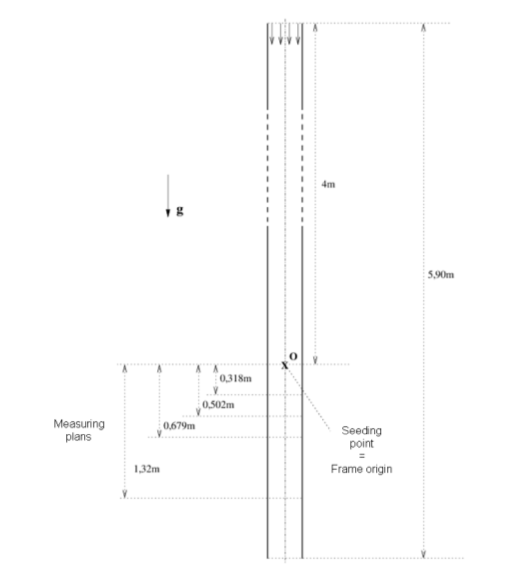
\includegraphics[width=10cm]{\IMAGES/Part2_Particle_dispersion/Schema_Arnason.png}
\caption{Schematic description of the Arnason experimental set-up \cite{Arnason}}\label{lag:Schema_Arnason}
\end{figure}

The dimensions of the pipe and the distance from the air inlet to the injection point are listed in \tablename~\ref{lag:pipe_dim} for clarity.

\begin{table}[H]
\begin{center}
\begin{tabular}{c p{4cm} c}
\Mline
\bf Pipe Internal  & \multicolumn{1}{c}{\multirow{2}{*}{\bf Pipe Length(m)}} & \bf Distance from Inlet  \\
\bf Diameter(m) & & \bf to Injection (m) \\
\hline\hline
$0.09$ & \multicolumn{1}{c}{$5.9$} & $4.0$ \\
\Mline
\end{tabular}
\caption{Arnason pipe dimensions.\label{lag:pipe_dim}}
\end{center}
\end{table}

As can be seen in \figurename~\ref{lag:Schema_Arnason}, four measuring planes were used to obtain measurements of the air flow and the glass beads.  These four planes are located downstream of the bead injection point with their positions relative to this point listed in \tablename~\ref{lag:measurement_plane}.

\begin{table}[H]
\begin{center}
\begin{tabular}{c p{6cm}}
\Mline
\bf Plane & \multicolumn{1}{c}{\bf \ \ \ \ \ Distance from injector(m) \ \ \ \ \ } \\
\hline\hline
$1$ & \multicolumn{1}{c}{$0.318$} \\  
$2$ & \multicolumn{1}{c}{$0.502$} \\ 
$3$ & \multicolumn{1}{c}{$0.679$} \\ 
$4$ & \multicolumn{1}{c}{$1.320$} \\                 
\Mline
\end{tabular}
\caption{Distance of the measuring planes downstream of the injector.\label{lag:measurement_plane}}
\end{center}
\end{table}

The flow physics are described next.



\subsection{Flow Physics}


The flow in the pipe is incompressible, fully developed, turbulent, with the air carrier phase transporting and diffusing a second phase.  Given that the second phase is dilute with respect to the carrier fluid, it is possible to assume that the glass beads are influenced by the flow of air but have no influence on the magnitude and flow direction of the carrier fluid.  This simplified modelling is known as one-way coupling.

The test rig operating conditions are described next.


\subsection{Operating Conditions}


The experimental test rig was operating with the following conditions:

\begin{itemize}
\item The maximum air velocity is of the order of 9.56m/s
\item The Reynolds number based on this maximum velocity is $50 \times 10^{3}$
\item The Reynolds number based on the mean velocity is $42\times 10^{3}$
\end{itemize}

The air temperature at inlet to the pipe is not provided in \cite{Arnason} so it is assumed to be $10^{\circ}C$.

Two sets of experiments are carried out with two different sets of glass beads and identical carrier fluid conditions.  The first set uses a bead diameter of $5\mu m$ and the second set a bead diameter of $57\mu m$.

The fluid properties are described next.


\subsection{Fluid Properties}

The fluid properties at the inlet temperature of $10^{\circ}C$ are listed in \tablename~\ref{lag:fluid_prop}.



\begin{table}[H]
\setlength\extrarowheight{5pt}
\begin{center}
\begin{tabular}{c c}
\Mline
\multirow{1}{*}{\bf $\rho (kg/m^3)$} & \multirow{1}{*}{\bf $\mu(Pa.s)$} \\
\hline\hline
\multirow{1}{*}{$1.2361$} & \multirow{1}{*}{$1.78*10^{-5}$} \\                  
\Mline
\end{tabular}
\caption{Fluid properties.\label{lag:fluid_prop}}
\end{center}
\end{table}

The properties of the glass beads are described next.



\subsection{Glass Beads} \label{lag:glass_beads}

The properties of the $5\mu m$ glass beads are listed in \tablename~\ref{lag:bead_prop}.

\begin{table}[H]
\setlength\extrarowheight{5pt}
\begin{center}
\begin{tabular}{c p{6cm} c}
\Mline
\multirow{1}{*}{\bf Mean diameter} & \multicolumn{1}{c}{\multirow{1}{*}{\bf \ \ \ \ Diameter Deviation \ \ \ \ }} & \multirow{1}{*}{\bf Density}\\
\multirow{1}{*}{\bf $d_p^{\mu}(\mu m)$} & \multicolumn{1}{c}{\multirow{1}{*}{\bf $\sigma_p(\mu m)$}} & \multirow{1}{*}{$\rho (kg/m^3)$} \\
\hline\hline
\multirow{1}{*}{$5.0$} & \multicolumn{1}{c}{\multirow{1}{*}{$1.0$}} & \multirow{1}{*}{$2475$} \\                  
\Mline
\end{tabular}
\caption{Glass bead properties.\label{lag:bead_prop}}
\end{center}
\end{table}

The particle diameter $d_p$ is calculated from the mean diameter and the deviation by $d_p=d_p^{\mu}+\varepsilon*\sigma_p$, where $\varepsilon$ is a random variable which follows a normal law.

The boundary conditions are discussed next.

\subsection{Boundary Conditions}

Three carrier fluid boundary conditions are used in this study: inlet, outlet and wall.  For the particles, the only boundary condition used is wall. \figurename~\ref{lag:Location_BC} illustrates the location of these boundary conditions and the flow direction (blue arrows).

\begin{figure}[H]
\centering
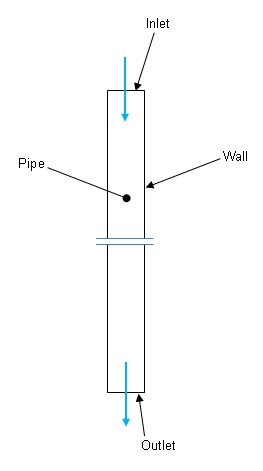
\includegraphics[width=5cm]{\IMAGES/Part2_Particle_dispersion/location_BC_crop.png}
\caption{Location of the boundary conditions.}\label{lag:Location_BC}
\end{figure}

\tablename~\ref{lag:bc_air_part} lists the various boundary values applied for the carrier fluid (air) and the particles.

\begin{table}[H]
\begin{center}
\begin{tabular}{c | c p{3cm} c}
\Mline
\bf Phase & \multicolumn{3}{c}{\bf \ \ \ \ \ \ \ \ \ \ \ \ \ Boundary Conditions and Values}   \\
 & \bf Inlet & \multicolumn{1}{c}{\bf Outlet} & \bf Wall \\
\hline\hline
\multirow{4}{*}{\bf Air} & \multicolumn{1}{l}{$u=0$} & \multicolumn{1}{c}{\multirow{4}{*}{Standard}}& \multirow{4}{*}{Wall} \\
 &\multicolumn{1}{l}{$v=0$}& & \\
 &$w=-V_{max}(1.0-\dfrac{0.4 \times r^2}{0.002025}) $& & \\
 &\multicolumn{1}{l}{$D_h=0.09m$}& & \\ 
\bf Particles & - & \multicolumn{1}{c}{-} & Rebound \\                  
\Mline
\end{tabular}
\caption{Boundary conditions and values for the air and the particles.\label{lag:bc_air_part}}
\end{center}
\end{table}

The inlet boundary condition corresponds to a Reynolds number of 42000 based on the mean velocity which itself corresponds to a mass flow rate of 0.06291kg/s.  A correction factor of 1.0488 is used to maintain the Reynolds number.

In the Arnason experiment, the particles are injected along the centre line of the pipe at the reference point.  Since the particle injection velocity is not given in \cite{Arnason}, in this tutorial we assume that it is equal to the local fluid velocity.

Also, the results presented in \cite{Arnason} do not stipulate the number of particles injected, the results only give statistical data.  For the simulations in this tutorial, 1000 particles are injected per time step in order to have a sufficient number of particles to post process.

Lastly, in the CFD model the turbulence at the inlet boundary is calculated directly by \CS using the hydraulic diameter, $D_h$, specified.

\subsection{One-Way Coupling CFD Modelling}\label{lag:one_way}

The one-way coupling simulation of the two-phase flow of the air and the glass beads is broken into two steps.  First, the flow of air alone is simulated.  This will be used as the background flow on which the particles are injected.  Then, in the second step, the flow of the particles on top of this air flow field is calculated.

\subsection{Creating \CS Study}\label{lag:create_CS_struct}

A \CS study called \textit{ARNASON} and a first case are created. This first case will be set up as a single-phase calculation. Call it \textit{RANS\_rij\_SSG}.

The study and the case are created using the procedure described in Part I of tutorial 1 \cite{ShearDriven_Tuto}.  Start \salome\_CFD, select the CFDStudy module, and go through all the steps detailed in \cite{ShearDriven_Tuto} to:

\begin{itemize}
\item Create the CFD study/case structure with the CFDStudy module
\item Save the new file as 'ARNASON'
\end{itemize}


\begin{figure}[h]
	\begin{minipage}[c]{.46\linewidth}
		\centering
		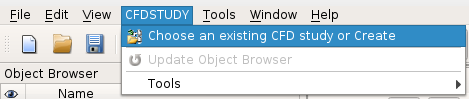
\includegraphics[scale = 0.6]{\IMAGES/create_cfd_study_salome8.png}
		\caption{\textit{Create a CFD study}}
		\label{lag:create_cfd.png}
	\end{minipage}
	\hfill%
	\begin{minipage}[c]{.40\linewidth}
		\centering
		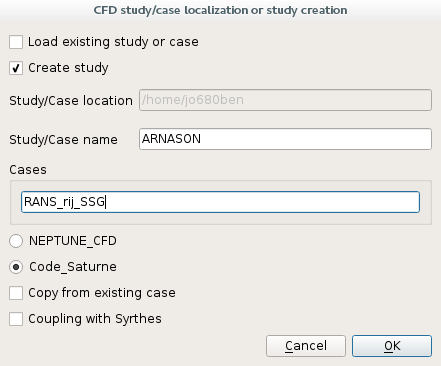
\includegraphics[scale = 0.5]{\IMAGES/cfd_study_salome8.png}
		\caption{\textit{CFD study localization or creation}}
		\label{lag:cfd_study}
	\end{minipage}
\end{figure}


In the end, you should end up with the directory structure (\figurename~\ref{lag:arbre_cfd_study}) shown in the Object Browser tab, displaying the study and the first case.

\begin{figure}[H]
	\centering
	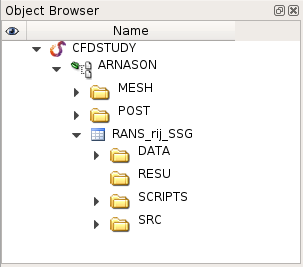
\includegraphics[scale=0.7]{\IMAGES/arbre2_salome8.png}
	\caption{\textit{ARNASON} Study, \textit{RANS\_rij\_SSG} case File Structure}\label{lag:arbre_cfd_study}
\end{figure} 

The case is then ready to be set up.
